\section{Data driven methods}
In this section, we will go through a different learning-based approach that has been explored in recent years. Learning-based methods in the field of social navigation can be broadly classified into reinforcement learning (RL)-based approach and inverse reinforcement learning(IRL)-based approaches. While these methods differ at their core, the problem definition for both the cases is similar but with a key difference. For both RL and IRL settings, the problem at hand is expressed in the form of a Markov decision process (MDP). We define the problem below.
\subsubsection*{Problem definition:}
\textbf{A Markov decision process is a discrete time stochastic control process $s^{*taken\ from\ wiki}$} and can be represented as a 4 tuple
($\mathcal{S}$,$\mathcal{A}$,T,$\gamma$, $\mathcal{R}$), where,
\begin{itemize}
	\item $\mathcal{S}$ is the set of all possible states.
	\item $\mathcal{A}$ is the set of all possible actions.
	\item T is the transition dynamics.
	\item $\gamma$ is the discount factor.
	\item $\mathcal{R}$ is the set of rewards.
\end{itemize}  
In a reinforcement learning problem setting, the goal is to find a policy $\pi$, which is a function that maps a state to action that maximizes the expected reward obtained.\\
In contrast, in an inverse reinforcement learning problem setting, there is no reward function provided. Instead, we are provided with a set of expert demonstrations say D = \{$\tau_1$, $\tau_2$, ... \}. And the goal is to generate a reward function $\mathcal{R}$, that best explains the expert behavior and a policy that would maximize the reward function.


\subsection*{RL based approaches}
 In their work, \textbf{Socially aware motion planning with Deep RL, Chen et. al.} address this problem by focusing on what not to do, rather than what to do. They introduce a reward function crafted to induce social norms in the behavior of the agent. The reward function primarily focuses on three different aspects of interaction: overtaking, passing and crossing as shown in the figure below.
 \begin{figure}[!htbp]
 	\centering
	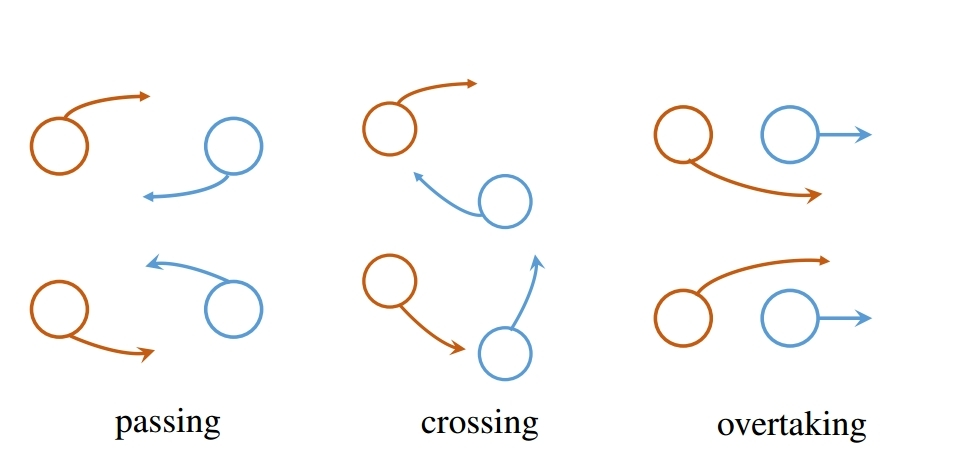
\includegraphics[width=.6\linewidth]{figures/chapter2_rl_based_approach}
 \end{figure}
\\
They note that symmetry is one of the driving factors to incorporate social behavior, so they introduce a network architecture for symmetric multi-agent training.\\

A more recent work by the same authors,\textbf{Collision avoidance in pedestrian-rich environments with deep reinforcement learning}
address some drawback of their previous work: the inability to tackle variable number of agents in the environment. They introduce a Long Short-Term Memory (LSTM) based network architecture that takes as input the information from the nearby pedestrians in a sequence. This eliminates the need for specifying a limit on the number of nearby-agents the method can handle.\\
The state comprises of two parts: 
\begin{enumerate}
	\item The information of the agent itself, \textbf{s}
	\item The information from the other n number of agents present in the environment at a given time. This is where the LSTM comes in to play which takes the information from these n agents and passes them sequentially through an LSTM layer to generate a final hidden state which is concatenated with \textbf{s} to obtain the final state representation of the environment.
\end{enumerate}
\begin{figure}[!htbp]
	\centering
	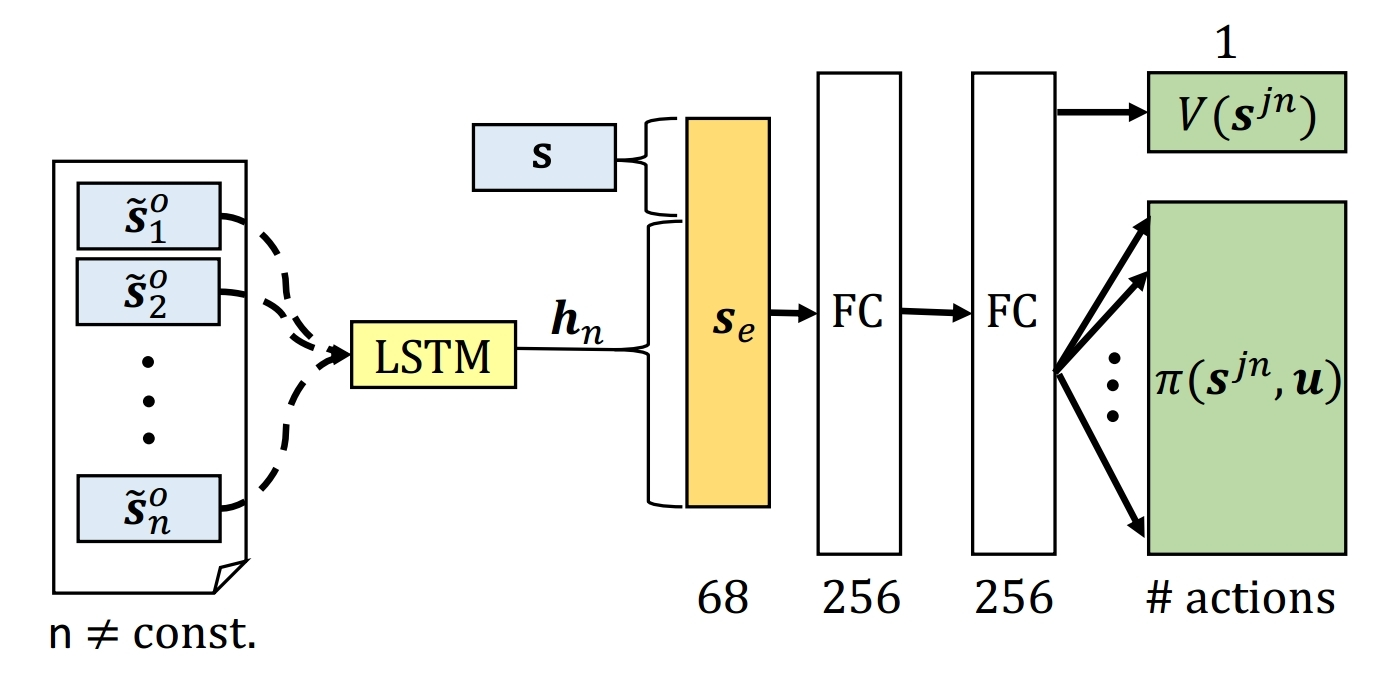
\includegraphics[width=0.6\linewidth]{figures/everett}
\end{figure}

The reward function used in this work is a relatively straight forward sparse reward structure with positive and negative feedback for reaching the goal or encountering a collision respectively.

\textbf{Conclusion}\\
Reinforcement learning, as a class of methods, has been widely successful in solving various complex control tasks including but not limited to video games making it one of the more obvious choices to tackle the problem of social navigation. 
However, using RL in this particular setting necessitates the formulation of a reward function that can correctly capture the 'social and cultural' characteristics. Coming up with such a set of rules can be difficult and daunting as 'social norms' are not always explicit and can vary widely across different societies and even based on a given situation.\\

\subsection*{IRL based approaches}
\textbf{Learning approaches meet probabilistic road map style path planner.}

\textbf{Vasquez et al} in their work, present a comprehensive study on the effect of different feature representations and IRL methods on the performance of an agent in the task of social navigation. They examine two IRL methods:
max-margin IRL and max entropy IRL.\\
For the feature representations, they create a pool of measurements garnered from the state of the agent itself and the state of the other entities in the environment and combine these measurements to create 3 feature representations. \\
They test all of these on a ROS based pedestrian simulator on 3 scenarios: airport gate, crossing hallway, and intersection. Expert demonstrations for these scenarios are obtained through tele-operation. They find that the performance across the two learning methods are similar. The feature representation, on the other hand, plays a major role in the final performance of the agent hence they come to the conclusion that spending time on modeling the feature representations or working to come up with learning methods that aid in the simplification of building the feature representations might be the way to go.\\

\textbf{Kim and Pineau} in their work, Socially adaptive path planning, present a way to automate the navigation of a wheelchair in a social setting. Their navigation framework comprises of 3 components, the feature extractor, the IRL module, and the path planner.\\
\textbf{Feature extractor}
The features are generated from the readings of an RGB-d sensor (3d point cloud) mounted on the robot. The area around the agent is divided into 3d blocks or cells and the features are calculated for each of these spatial cells. 
The authors calculate 4 features namely,
crowd density, speed, velocity and distance to the goal.
While the calculation of the crowd density and the distance to the goal are straight forward, the calculation of the speed and velocity from 3d point clouds are more involved and the authors use an RGB-d optical flow method based on Farneback RGB optical flow. 
\\ \textbf{The optical flow algorithm??}
The result is a 12-dimensional binary feature vector for each grid cell.
\textbf{IRL module}
The authors use Maximum a posterior i Bayesian Inverse reinforcement learning (MAP-BIRL) to calculate the cost function for socially acceptable navigation. Cost of a given state is given by
\begin{align}
C(s,a) = \sum^{d}_{i=1} w_i \phi_i(s,a)
\end{align}
where the weight vector w is learned from MAP-BIRL. 
The weight vector is obtained by obtaining the MAP inference of the following expression:
\begin{align}
L(w) = \sum^M_{m=1} \sum^{H}_{h=1}log[\frac{\exp \mathcal{Q}^{*}_m(s^m_h, a^m_h)}{\sum_{a\in A} \exp(\mathcal{Q}_m^*(s_h^m,a))}]
\end{align}
For the path planning, the authors maintain a hierarchical path planner consisting of 3 parts: global planner, local planner, and a collision detector.
The global planner chalks out a global path from the starting position of the robot to the goal state. The entire path is broken down into multiple sub-goals and the responsibility of moving from one sub-goal to the next falls on the local planner. During the run, the planner maintains a collision detector based on handcrafted rules.
The authors test their method on different scenarios including one that involves the robot operating in a crowded corridor.\\

In one of the more recent works by \textbf{Fahad et. al.}, they present a navigation framework to train agents from demonstrations using maximum entropy Deep IRL where, the objective is to maximize the likelihood of the states visited by the expert.
This is achieved by dividing each demonstration, or trajectory, in this case, into a sum of the individual states encountered by the expert. and minimizing the difference in the state visitation frequency (SVF) of the agent and the expert.\\
The authors present a feature representation consisting of 4 parts:
\begin{enumerate}
	\item Social Affinity Map feature(SAM): This captures the motion of the pedestrians in the vicinity of the agent. The area near the agent is divided into two concentric circles. The region inside the inner circle is then divided into 4 parts, and the region between the inner and outer circle is divided into 6 parts.
	Information from each of these 10 areas (or bins) is then expressed using a 6-dimensional vector that captures the average velocity of the pedestrians in a given bin. 
	\item Density feature: Helps provide an idea of how dense the vicinity of the agent is. It is calculated by adding up the number of pedestrians present in the spatial bins (calculated above). Once calculated they are discretized based on some predefined threshold.
	\item Distance feature: Captures the distance between the agent's current location and the goal.
	\item Default Cost feature: Introduced to balance the rest of the other features. This has been proposed by various other works in the past.
	
\end{enumerate}
The authors train and test their procedure using data collected in the "ATC" business center in Osaka, Japan.
From these experiments they show that the method is not only capable of producing a general navigator to negotiate the crowd, but also an agent that show traits of pedestrian behaviors like collision-avoidance and following the leader.


\textbf{Conclusion:}
Given the nature of the task, IRL based methods seem to be a promising avenue to explore. But the problem of social navigation is far from solved and there are many issues that still need addressing. IRL methods are highly dependent on the design of the feature representation used in the algorithm, and a lot of time and effort are needed towards optimizing a set of features that would perform well. Moreover, for most of the existing work not a lot has been discussed about generalization of the agent. Most of the experiments are either conduced in a relatively simple environment, like a narrow hallway or address some specific aspect of crowd navigation like negotiating intersections. 
\begin{comment}
\textbf{Collection of expert trajectory might be expensive}
\textbf{The generalization of the method is not that great for now}
\textbf{The dependence of IRL on feature engineering: IRL methods are highly dependent on the design of the feature representation used in the algorithm, and a lot of time and effort are needed towards optimizing a set of features that would perform well.}

The primary advantage of IRL over the other methods discussed, both model-based and data-driven methods, is that there is no need to specify a handcrafted reward function built to induce certain kinds of behavior within the agent. Most of the current work in this domain primarily focuses on capturing the expert's behavior, thus encapsulating the 'naturalness' in the movements during navigation.
Disadvantages:
Comment of IRL and feature engineering. 
Getting expert demonstrations are more expensive compared to RL.
Hard to generalize. 
\end{comment}